% +--------------------------------------------------------------------+
% | Appendix A Page (Optional)                                         
% +--------------------------------------------------------------------+

\cleardoublepage

\chapter{Experiment Documentation}

\label{Appendix:Key1}

\begin{figure}[htb]
	\centering
	\subfloat[300 RPM]{
		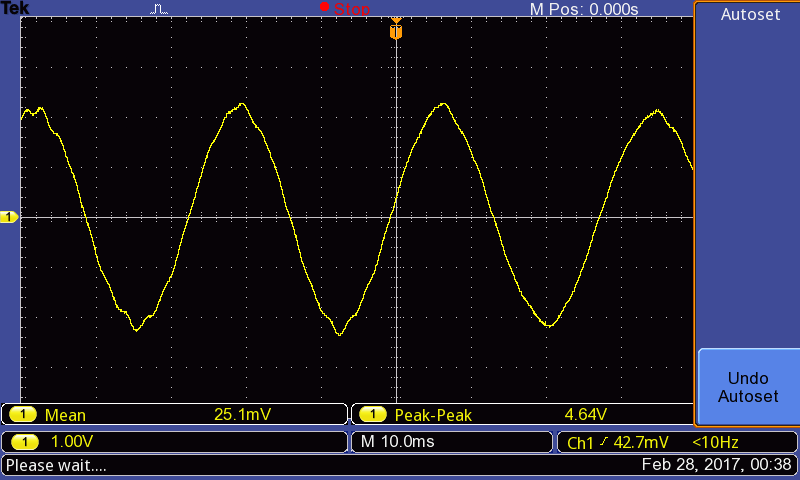
\includegraphics[width=55mm]{figures/appendix/TEK2.png}
	}
	\subfloat[500 RPM]{
		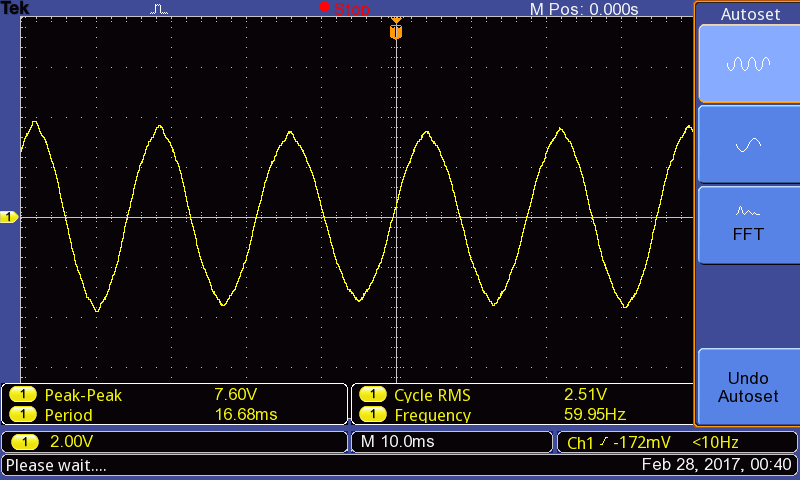
\includegraphics[width=55mm]{figures/appendix/TEK3.png}
	}
	\newline
	\subfloat[1000 RPM]{
		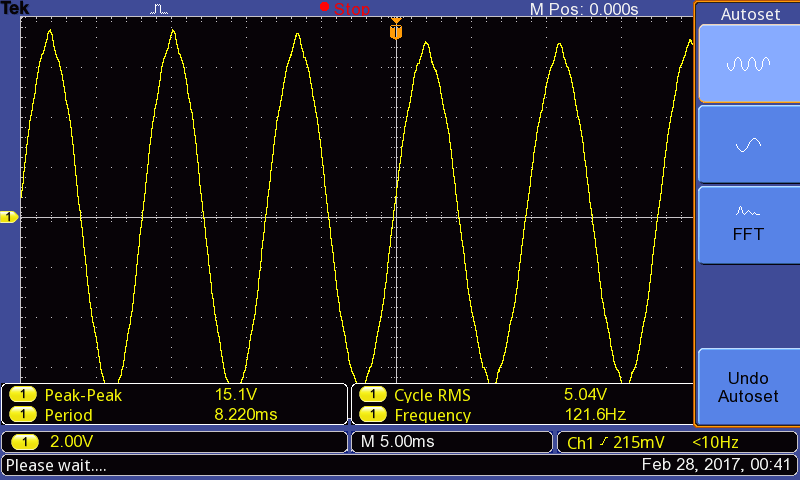
\includegraphics[width=55mm]{figures/appendix/TEK4.png}
	}
	\subfloat[1500 RPM]{
		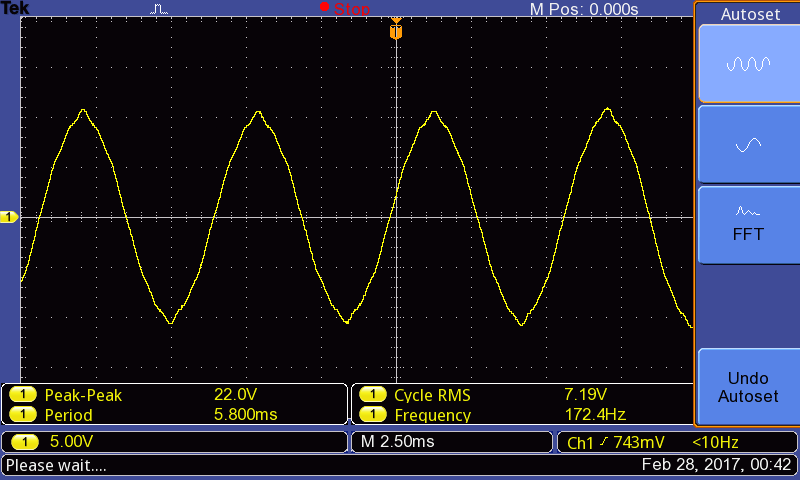
\includegraphics[width=55mm]{figures/appendix/TEK5.png}
	}
	\newline
	\hbox to 0mm{}% !!
	\subfloat[2000 RPM]{
		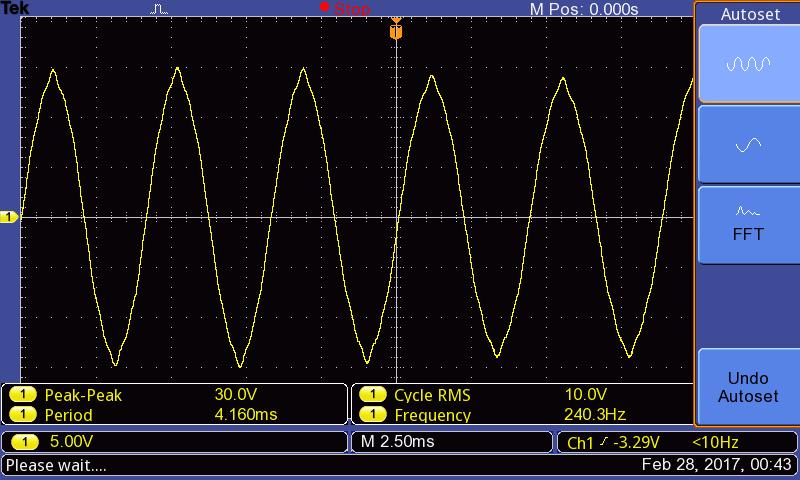
\includegraphics[width=55mm]{figures/appendix/TEK6.png}
	}
	\caption{Back emf at various motor speeds}
	\label{back_emf_measurement}
\end{figure}

\begin{table}[ht]
	\begin{center}
		\caption{NERMLAB Parameters}
		\begin{tabular}{|M{3cm}|M{3cm}|M{3cm}|M{3cm}|N}
			
			\hline
			\textbf{Parameter} & \textbf{Description} & \textbf{Value} & \textbf{Units}\\
			
			\hline
		    J & Lumped Inertia ($J_w + J_r$)  & $1.8757\times10^{-5}$ & $kg\cdot m^2$ &\\[25pt]
			
			\hline
			$J_w$ & Washer Inertia & $1.4256\times10^{-5}$ & $kg\cdot m^2$ &\\[25pt]
			
			\hline
			$J_r$ & Rotor Inertia & $4.5013\times10^{-6}$ & $kg\cdot m^2$ &\\[25pt]
			
			\hline
			$b$ & Viscous Friction & $5.3\times10^{-4}$ & $\frac{N\cdot m \cdot s}{rad}$ &\\[25pt]
			
			\hline
			$k_T$ & Motor Torque Constant & $0.0617$ & $\frac{N\cdot m}{A}$ &\\[25pt]
			
			\hline
			$L$ & Motor Inductance & $-$ & $H$ &\\[25pt]
			
			\hline
			$R$ & Motor Phase Resistance & $5$ & $\Omega$ &\\[25pt]
			
			\hline
			$K_{e,LL}$ & Back-EMF Constant & $0.0713$ & $\frac{V\cdot s}{rad}$ &\\[25pt]
			
			\hline
		\end{tabular}
		
		\label{NERMLAB_PARAMETERS}
	\end{center}
\end{table}